\begin{figure}[h!]
	\centering
	
	
	
	\tikzset{every picture/.style={line width=0.75pt}} %set default line width to 0.75pt        
	
	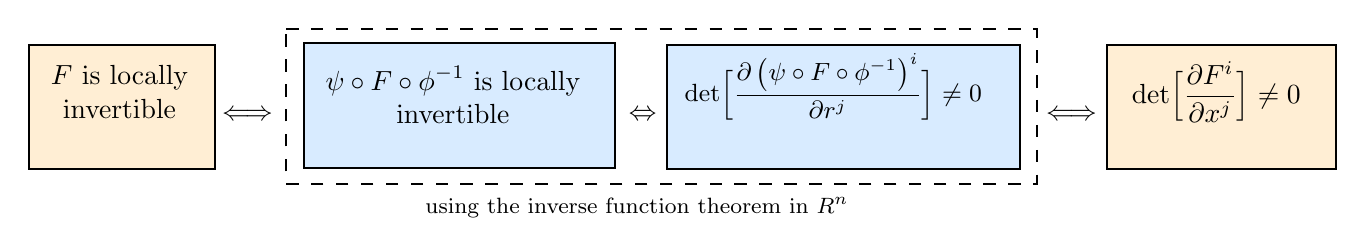
\begin{tikzpicture}[x=0.75pt,y=0.75pt,yscale=-1,xscale=1]
		%uncomment if require: \path (0,300); %set diagram left start at 0, and has height of 300
		
		%Shape: Rectangle [id:dp28925530323831317] 
		\draw  [fill={rgb, 255:red, 154; green, 203; blue, 255 }  ,fill opacity=0.39 ] (143,39.33) -- (292.67,39.33) -- (292.67,99.33) -- (143,99.33) -- cycle ;
		%Shape: Rectangle [id:dp34966788396180615] 
		\draw  [fill={rgb, 255:red, 154; green, 203; blue, 255 }  ,fill opacity=0.39 ] (318,40) -- (488,40) -- (488,100) -- (318,100) -- cycle ;
		%Shape: Rectangle [id:dp8415325367676847] 
		\draw  [fill={rgb, 255:red, 255; green, 203; blue, 120 }  ,fill opacity=0.32 ] (10.33,40) -- (100,40) -- (100,100) -- (10.33,100) -- cycle ;
		%Shape: Rectangle [id:dp9745265751684289] 
		\draw  [fill={rgb, 255:red, 255; green, 203; blue, 120 }  ,fill opacity=0.32 ] (530,40) -- (640,40) -- (640,100) -- (530,100) -- cycle ;
		%Shape: Rectangle [id:dp35176055981313437] 
		\draw  [dash pattern={on 4.5pt off 4.5pt}] (134.33,32.33) -- (496,32.33) -- (496,107) -- (134.33,107) -- cycle ;
		
		% Text Node
		\draw (17,48.67) node [anchor=north west][inner sep=0.75pt]   [align=left] {\begin{minipage}[lt]{53.36pt}\setlength\topsep{0pt}
				\begin{center}
					$\displaystyle F$ is locally \\invertible
				\end{center}
				
		\end{minipage}};
		% Text Node
		\draw (148,49) node [anchor=north west][inner sep=0.75pt]   [align=left] {\begin{minipage}[lt]{97.77pt}\setlength\topsep{0pt}
				\begin{center}
					$\displaystyle \psi \circ F\circ \phi ^{-1}$ is locally \\invertible
				\end{center}
				
		\end{minipage}};
		% Text Node
		\draw (319,43) node [anchor=north west][inner sep=0.75pt]  [font=\small] [align=left] {\begin{minipage}[lt]{116.2pt}\setlength\topsep{0pt}
				\begin{center}
					$\displaystyle \det\Bigl[\frac{\partial \left( \psi \circ F\circ \phi ^{-1}\right)^{i}}{\partial r^{j}}\Bigr] \neq 0$ 
				\end{center}
				
		\end{minipage}};
		% Text Node
		\draw (531.67,46.67) node [anchor=north west][inner sep=0.75pt]   [align=left] {\begin{minipage}[lt]{74pt}\setlength\topsep{0pt}
				\begin{center}
					$\displaystyle \det\Bigl[\frac{\partial F^{i}}{\partial x^{j}}\Bigr] \neq 0$ 
				\end{center}
				
		\end{minipage}};
		% Text Node
		\draw (298,70) node [anchor=north west][inner sep=0.75pt]    {$\Leftrightarrow $};
		% Text Node
		\draw (200,112) node [anchor=north west][inner sep=0.75pt]  [font=\footnotesize] [align=left] {using the inverse function theorem in $\displaystyle \mathbb{R}^{n}$};
		% Text Node
		\draw (102,70) node [anchor=north west][inner sep=0.75pt]    {$\Longleftrightarrow $};
		% Text Node
		\draw (499,70) node [anchor=north west][inner sep=0.75pt]    {$\Longleftrightarrow $};
		
		
	\end{tikzpicture}
\end{figure}